\documentclass[12pt, twoside]{article}
\usepackage[letterpaper, margin=1in, headsep=0.5in]{geometry}
\usepackage[english]{babel}
\usepackage[utf8]{inputenc}
\usepackage{amsmath}
\usepackage{amsfonts}
\usepackage{amssymb}
\usepackage{tikz}
\usetikzlibrary{quotes, angles}
\usepackage{venndiagram}
\usepackage{multicol}

\usepackage{fancyhdr}
\pagestyle{fancy}
\fancyhf{}
\renewcommand{\headrulewidth}{0pt} % disable the underline of the header

%\fancyhead[RE]{\thepage}
%\fancyhead[RO]{\thepage \\ Name: \hspace{3cm}}
%\fancyhead[L]{BECA / Dr. Huson / IB Math\\* 7 October 2019}


\begin{document}
\subsubsection*{2.2 Applications of the laws of sines and cosines}

\begin{enumerate}

  \item Express each value as a decimal, first writing the whole calculator display, and then the 3 sig-fig approximation. \hfill [4 marks]
  \begin{multicols}{2}
    \begin{enumerate}
    \item $\displaystyle \frac{2\pi}{3}$
    \item $\displaystyle \frac{\sqrt{3}}{2}$
    \end{enumerate}
  \end{multicols} \vspace{2cm}

  \item Express each value as a decimal, rounding to 3 sig-figs if necessary. \hfill [3 marks]
  \begin{multicols}{2}
    \begin{enumerate}
    \item $4.561 \times 10^4$
    \item $1.90 \times 10^{-3}$
    \end{enumerate}
  \end{multicols}

  \newpage
  \item $\triangle ABC$ is shown with $m\angle C=90^\circ$ and the lengths of the triangle's sides are $BC=8$, $AC=6$, and $AB=10$.
  \begin{multicols}{2}
        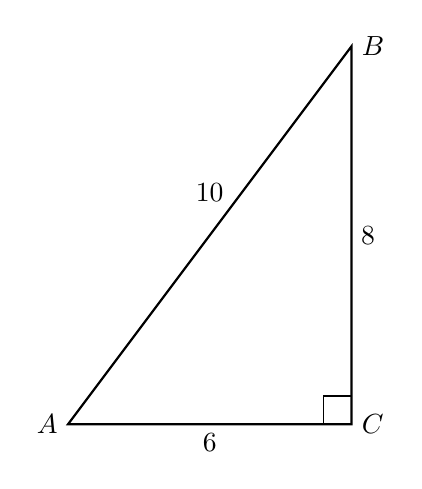
\begin{tikzpicture}[scale=0.6]
          \draw [thick]
          (0,0)node[left]{$A$}--
          (6,0)node[ right]{$C$}--
          (6,8)node[right]{$B$}--cycle;
          \draw (6,0)++(-0.6,0)--++(0,0.6)--+(0.6,0);
          \node at (3,0)[below]{$6$};
          \node at (6,4)[right]{$8$};
          \node at (3,4.5)[above]{$10$};
        \end{tikzpicture}
        \begin{enumerate}
        \item Write down the value of $\sin A$.  \\ \hfill [1 mark]\vspace{2cm}
        \item Find the measure of $\angle A$.  \hfill [2 marks] \vspace{1cm}
      \end{enumerate}
    \end{multicols}

\newpage
   \item In right triangle $ABC$, hypotenuse $\overline{AB}$ has a length of 26 cm, and side $\overline{BC}$ has a length of 17.6 cm. What is the measure of angle $B$?

\newpage
\subsubsection*{Triangle area sine formula}
   \item Find the area of triangle $ABC$, with $AB=15$, $AC=17$, $m\angle A = 52^\circ$. \\[0.5cm]
   Hint: To use the area formula $A = \frac{1}{2} bh$ first find the altitude using sine and the hypotenuse $AC=17$.
   \begin{flushleft}
     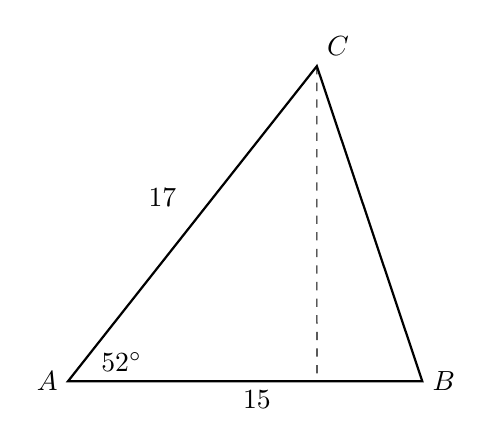
\begin{tikzpicture}[scale=0.3]
       \draw [-, thick] (51.7:17) node[above right]{$C$}--
         (0,0) node[left]{$A$}--
         (15,0) node[right]{$B$}--cycle;
       \node at (1, 0)[above right]{$52^\circ$};
       \node at (5, 7)[above left]{$17$};
       \node at (8, 0)[below]{$15$};

     \draw [-, dashed] (51.7:17)--(10.54,0);

     \end{tikzpicture}
     \end{flushleft} 

\newpage
\subsubsection*{Law of sines}
  \item Solve the given triangle (determine the values of all lengths and angles)
  \begin{center}
    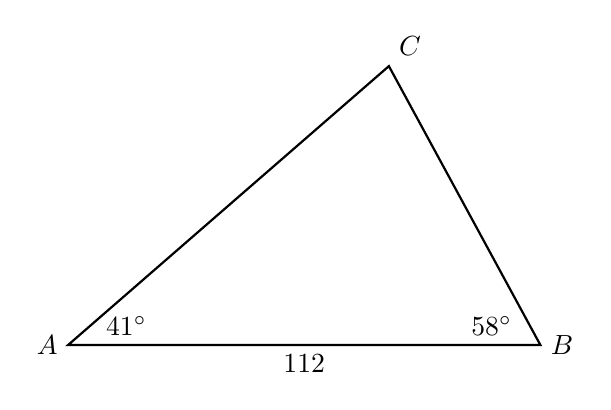
\begin{tikzpicture}[scale=1.2]
      \draw [-, thick] (41:4.5) node[above right]{$C$}--
        (0,0) node[left]{$A$}--
        (5,0) node[right]{$B$}--cycle;
      \node at (0.3, 0)[above right]{$41^\circ$};
      \node at (4.8, 0)[above left]{$58^\circ$};
      \node at (2.5, 0)[below]{$112$};
    \end{tikzpicture}
    \end{center}

\newpage
\subsubsection*{Law of sines}
  \item The following diagram shows triangle $ABC$ (not drawn to scale).
  \begin{center}
    \begin{tikzpicture}[scale=1.4, rotate=-25]
      \draw [-, thick] (50:3.5) node[above right]{$C$}--
        (0,0) node[left]{$A$}--
        (5,0) node[right]{$B$}--cycle;
      \node at (0.3, 0.15)[right]{$50^\circ$};
      \node at (4.5, 0.3)[above left]{$43^\circ$};
      \node at (3.7, 1.8)[below]{$11$};
    \end{tikzpicture}
    \end{center} 
    $BC=11$, $C\hat{A}B=50^\circ$, and $A\hat{B}C=43^\circ$
    \begin{enumerate}
      \item Find $AC$. \hfill [3 marks]
      \item Find the area of triangle $ABC$. \hfill [3 marks]
    \end{enumerate}

\newpage
  \item The following diagram shows quadrilateral $ABCD$ (not drawn to scale).
  \begin{center}
    \begin{tikzpicture}[scale=1.5, rotate=-20]
      \draw [-, thick] (100:3.5) node[above right]{$D$}--
        (0,0) node[below]{$B$}--
        (-5,0) node[below]{$A$}--cycle;
      \draw [-, thick] (100:3.5) --
      (55:3) node[right]{$C$}--
      (0,0);             
      \node at (58:2.9)[left]{$78^\circ$};
      \node at (50:1.5)[right]{$5.1$};
      \node at (-2.5,-0.2)[below]{$8.0$};
      \node at (78:3.5)[below]{$4.2$};
      \node at (-3,2.2)[below]{$8.3$};
    \end{tikzpicture}
    \end{center} 
    $AB=8.0$, $BC=5.1$, $CD=4.2$, $AD=8.3$, and $B\hat{C}D=78^\circ$
    \begin{enumerate}
      \item Find $BD$. \hfill [3 marks]
      \item Find $A\hat{B}D$. \hfill [3 marks]
    \end{enumerate}

\newpage
\subsubsection*{Precision application}
  \item BMI is a measure of a healthy personal weight, 
  \[\displaystyle BMI = \frac{w}{h^2}\]
    where \\
    $w$ is a person's weight in kilograms, and \\
    $h$ is height in meters
    \begin{enumerate} 
        \item Given a height of 160 cm and weight of 54 kg, find the BMI  \hfill [3 marks]
        \item These measurements are not exact. Assuming the height is between 159-161 cm and weight 53-55 kg, find the bounds of the BMI.  \hfill [4 marks]
      \end{enumerate}

\newpage
\subsubsection*{Sine ambiguous case}
  \item Triangle $ABC$ has an area of 25, with $AB=7$ and $AC=8$. 
  \begin{enumerate}
    \item Find the two possible measures for $\hat{A}$. \hfill [4 marks]
    \item Given that $\hat{A}$ is obtuse, find $BC$. \hfill [3 marks]
  \end{enumerate}

\newpage
\subsubsection*{Solid geometry}
\item Find the slant height of a pyramid with square base 4 meters on a side and height of 4 m. \hfill [3 marks]


  \item Find the volume of a spherical balloon 36 meters in diameter. \hfill [3 marks]
  
  \item A cone has a height of 24 cm and volume of $220.5\pi \,\mathrm{ cm}^3$. Find its radius. \hfill [3 marks]
  


\end{enumerate}
\end{document}
